\documentclass[compress]{beamer}
\usepackage{graphicx,amsmath,amsthm,verbatim,bm}
\usepackage{longtable}
%\usetheme{Copenhagen}
%\useoutertheme[{options}]{tree}
%\setbeamertemplate{footline}[page number]
%\useoutertheme{infolines}
%\setbeamertem plate{headlirne}{}
\useinnertheme{circles}
\usepackage{comment}
\setbeamertemplate{footline}[frame number]
%\usepackage{times}
%\usepackage[tbtags]{amsmath}
%\usepackage{amssymb}
\usepackage{amsfonts}
%\usepackage{slfortheorems}
\usepackage{epsfig}
\usepackage{graphicx}
\usepackage[small]{caption}
\usepackage[square]{natbib}
%\newcommand{\newblock}{}
\bibpunct{(}{)}{;}{a}{}{,}
\bibliographystyle{ims}
%\usepackage[letterpaper]{geometry}
\usepackage{color}
\setlength{\parindent}{0pt}
\usepackage{bbding}
\usepackage{long table, booktabs}



\usepackage{listings}
\usepackage[ruled,lined]{algorithm2e}
\def\algorithmautorefname{Algorithm}
\SetKwIF{If}{ElseIf}{Else}{if}{then}{else if}{else}{endif}

\usepackage{longtable}



\theoremstyle{plain}
\usepackage{amsfonts}
\usepackage{epsfig}
\usepackage{graphicx}
%\usepackage[small]{caption}

\usepackage{zref-savepos}

\newcounter{restofframe}
\newsavebox{\restofframebox}
\newlength{\mylowermargin}
\setlength{\mylowermargin}{2pt}

\newenvironment{restofframe}{%
    \par%\centering
    \stepcounter{restofframe}%
    \zsavepos{restofframe-\arabic{restofframe}-begin}%
    \begin{lrbox}{\restofframebox}%
}{%
    \end{lrbox}%
    \setkeys{Gin}{keepaspectratio}%
    \raisebox{\dimexpr-\height+\ht\strutbox\relax}[0pt][0pt]{%
    \resizebox*{!}{\dimexpr\zposy{restofframe-\arabic{restofframe}-begin}sp-\zposy{restofframe-\arabic{restofframe}-end}sp-\mylowermargin\relax}%
        {\usebox{\restofframebox}}%
    }%
    \vskip0pt plus 1filll\relax
    \mbox{\zsavepos{restofframe-\arabic{restofframe}-end}}%
    \par
}


\usepackage{tikz}
\usetikzlibrary{arrows}

%\usepackage[usenames,dvipsnames]{xcolor}
\usepackage{tkz-berge}
\usetikzlibrary{fit,shapes}

\usepackage{calc}
\usetikzlibrary{decorations.markings}

\tikzstyle{vertex}=[circle, draw, inner sep=0pt, minimum size=6pt]
\newcommand{\vertex}{\node[vertex]}
\newcounter{Angle}



%%%to add in new counter for slides in beamer
\newcommand{\beginbackup}{
   \newcounter{framenumbervorappendix}
   \setcounter{framenumbervorappendix}{\value{framenumber}}
}
\newcommand{\backupend}{
   \addtocounter{framenumbervorappendix}{-\value{framenumber}}
   \addtocounter{framenumber}{\value{framenumbervorappendix}} 
}


\newcommand*\oldmacro{}
\let\oldmacro\insertshortauthor
\renewcommand*\insertshortauthor{
  \leftskip=.3cm
\insertframenumber\,/\,\inserttotalframenumber\hfill\oldmacro}




\excludecomment{notbeamer}
\includecomment{beamer}

\newcommand{\lam}{\mathbf{\Lambda}}	
\newcommand{\bX}{\mathbf{X}}
\newcommand{\bY}{\mathbf{Y}}



\title[Entity Resolution: \\Measuring and Reporting Quality]
{Entity Resolution: \\Measuring and Reporting Quality}
\author[Rebecca C. Steorts, beka@stat.duke.edu]{Rebecca C. Steorts} 

\institute{\normalsize Department of Statistical Science, affiliated faculty in Computer Science, Biostatistics and Bioinformatics, the information initiative at Duke (iiD) and \\the Social Science Research Institute (SSRI) \\ Duke University and U.S. Census Bureau\\ \vspace*{1em}

\begin{figure}[htbp]
\begin{center}

\includegraphics{figures/banner}
%\caption{default}
\label{default}
\end{center}
\end{figure}}
\date{January 25, 2018}


\begin{document}
\begin{frame}
\titlepage
\end{frame}

\frame{
\begin{center}
\Large
\emph{Entity resolution (record linkage or de-duplication) joins multiple data sets removes duplicate entities often in the absence of a unique identifier.}
\end{center}

}

\begin{frame}
\frametitle{Motivations}
  \begin{columns}[T]
    \begin{column}{.5\textwidth}
     \begin{block}{In Syria, we have duplicated information regarding individuals who have died in the conflict. \\
\vspace*{2em}
   In the census, we have duplicated information of individuals that fill out census forms every 10 years. \\
\vspace*{2em}
Goal: Estimation of the sample size and associated standard errors. 
 }
% Your text here
    \end{block}
    \end{column}
    \begin{column}{.5\textwidth}
    \begin{block}{}
% Your image included here
    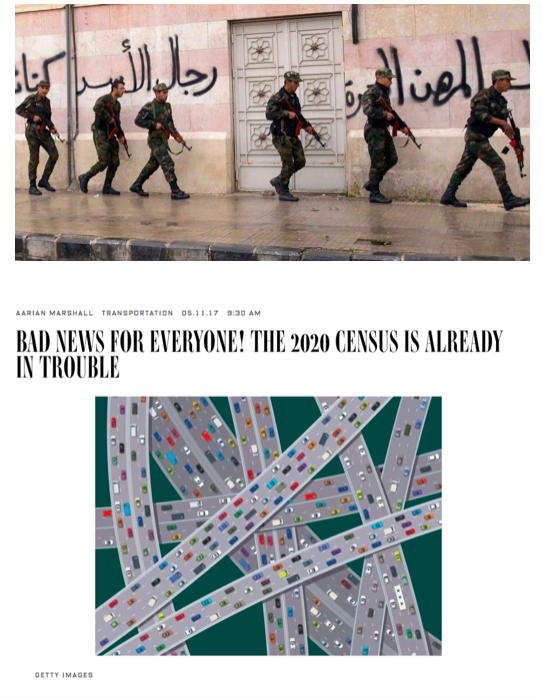
\includegraphics[width=\textwidth]{figures/syria-census2}
    \end{block}
    \end{column}
  \end{columns}
\end{frame}

\frame{
\frametitle{A graph with no edges}
\begin{figure}[htbp]
\begin{center}
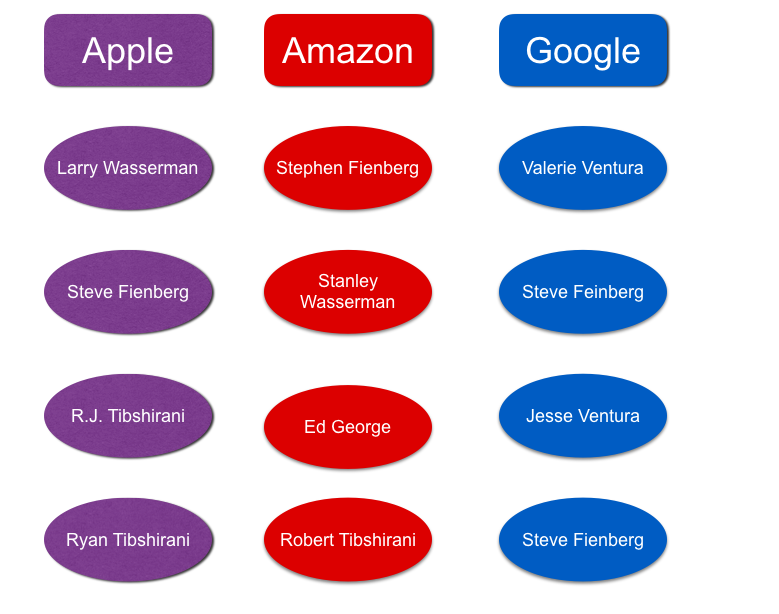
\includegraphics[scale=0.35]{figures/linkage}
%\caption{default}
%\label{default}
\end{center}
\end{figure}



}

\frame{
\frametitle{The record linkage graph}
\begin{figure}[htbp]
\begin{center}
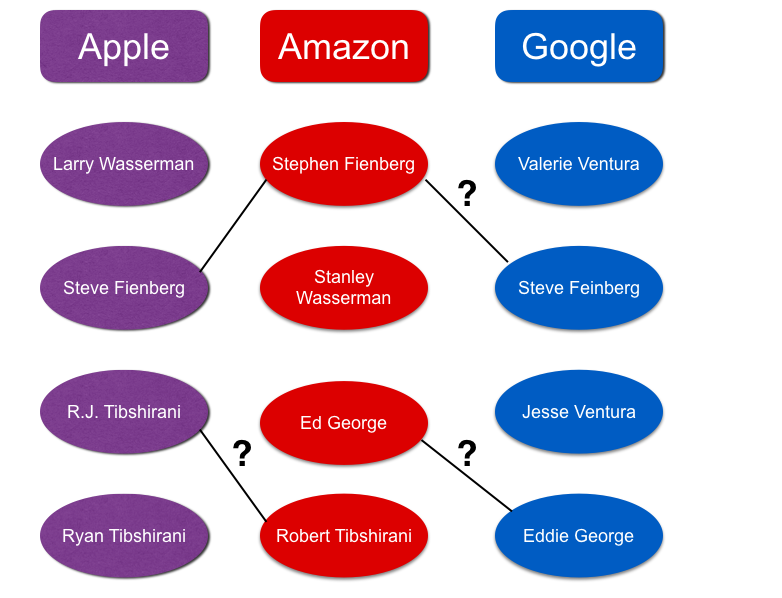
\includegraphics[scale=0.35]{figures/linkage2}
%\caption{default}
%\label{default}
\end{center}
\end{figure}

}

\frame{
\frametitle{The node of Larry Wasserman}
\begin{figure}[htbp]
\begin{center}
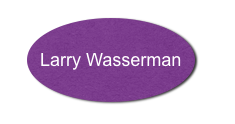
\includegraphics[scale=0.35]{figures/node}
%\caption{default}
%\label{default}
\end{center}
\end{figure}



}

\frame{
\frametitle{The node of Larry Wasserman}
\begin{figure}[htbp]
\begin{center}

\includegraphics[scale=0.35]{figures/node-feature}
%\caption{default}
%\label{default}
\end{center}
\end{figure}



}

\frame{
\frametitle{The record linkage graph}
\begin{figure}[htbp]
\begin{center}
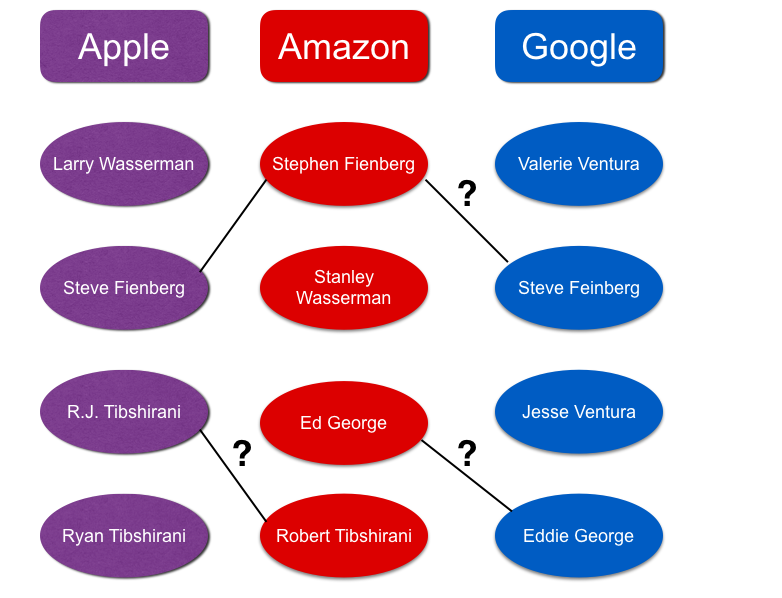
\includegraphics[scale=0.35]{figures/linkage2}
%\caption{default}
%\label{default}
\end{center}
\end{figure}

}

%\frame{
%
%If we had infinite time, we would make all-to-all record comparisons and remove the duplicate entities. 
%
%This is not tractable
%
%
%}

\frame{
\frametitle{Who's the real Steve Fienberg?}
\begin{figure}[ht]
\begin{minipage}[b]{0.45\linewidth}
\centering

\includegraphics[width=\textwidth]{figures/fienberg1}
%\caption{default}
%\label{fig:figure1}
\end{minipage}
\hspace{0.5cm}
\begin{minipage}[b]{0.45\linewidth}
\centering

\includegraphics[width=\textwidth]{figures/blank}
%\caption{default}
%\label{fig:figure2}
\end{minipage}
\end{figure}
}

\frame{
\frametitle{Who's the real Steve Fienberg?}

\begin{figure}[htbp]
\begin{center}
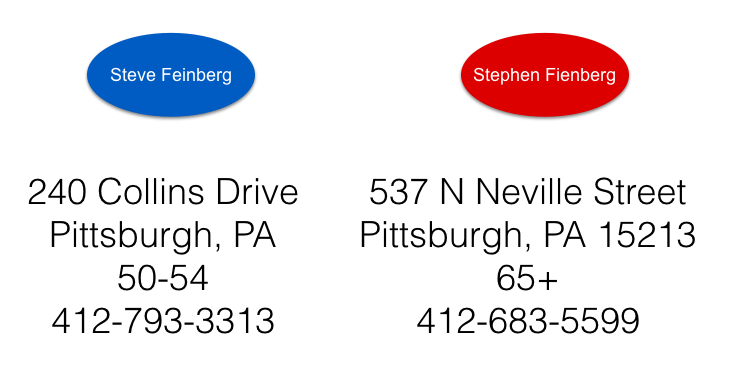
\includegraphics[width=\textwidth]{figures/fienberg}
\label{block}
\end{center}
\end{figure}


These are clearly not the \emph{same} Steve Fienberg!


}

%\subsection{Application to Syrian War}
\frame{
\frametitle{Syrian Civil War}
\vspace*{-0.75em}
\begin{figure}[htbp]
\begin{center}
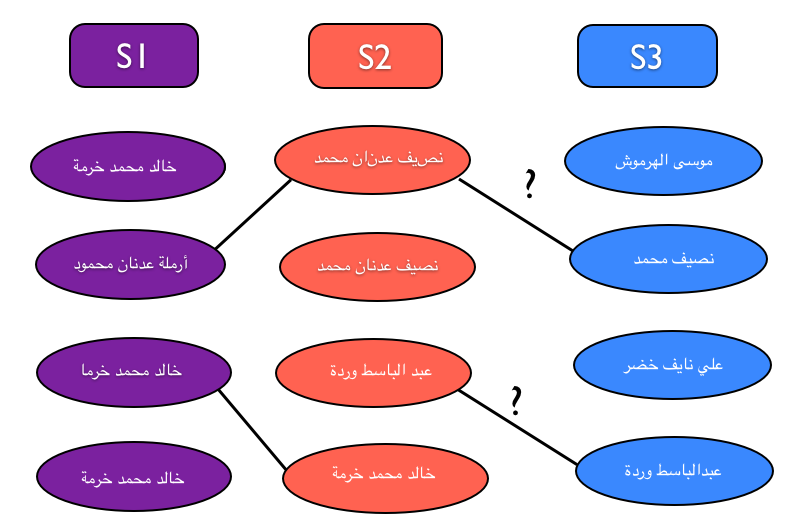
\includegraphics[scale=0.35]{figures/syrian}
%\caption{default}
%\label{default}
\end{center}
\end{figure}

%\begin{flushright}
%Steorts (2014, To be Submitted, AIStats)
%\end{flushright}



}





\frame{
\frametitle{Entity Resolution}
\Large
%\emph{Now, we can run any record linkage procedure in parallel once the blocks
%are created. How to do this?}\\

%\vspace*{1em}
\center
\emph{Why is entity resolution difficult?}

}


\frame{
\frametitle{Goals of Entity Resolution}

%\emph{Now, we can run any record linkage procedure in parallel once the blocks
%are created. How to do this?}\\

%\vspace*{1em}

Suppose that we have a total of $M$ records in $D$ data sets. 

\begin{enumerate}
\item We seek models that are much less than $O(M^2)$ (quadratic).
\item We seek models that are reliable, accurate, fit the data well, and account for the uncertainty of the model.
\end{enumerate}

\pause
These two goals fundamentally go against one another, making record linkage a very challenging problem.
\vspace*{1em}
\pause

%In this talk, we will focus on (2) since satisfying the above goals is very difficult. 

Depending on the motivating goal of a record linkage task, we approach it using either 1 or 2. 

}

\frame{

Suppose that we have a total of $M$ records in $D$ data sets. 

\begin{enumerate}
\item We seek models that are much less than $O(M^2)$ (quadratic).
\item We seek models that are reliable, accurate, fit the data well, and account for the uncertainty of the model.
\end{enumerate}

In the rest of the talk, we will
\begin{enumerate}
\item Review the literature.
\item Present Bayesian methods that satisfy 2.
\item And present a framework that satisfies both 1 and 2 (with a restriction). 
\end{enumerate}

}


\frame{
\frametitle{Terminology}

\begin{enumerate}
\item De-duplication
\item Record linkage
\item Blocking
\end{enumerate}


}

\frame{
\frametitle{De-duplication}

%De-duplication is the process where we ignore the uncertainty of the record linkage process. 
%
%\vspace*{1em}
%
%We combine the databases of Apple, Amazon, and Google and link records, assuming just one database. 

\begin{figure}[htbp]
\begin{center}
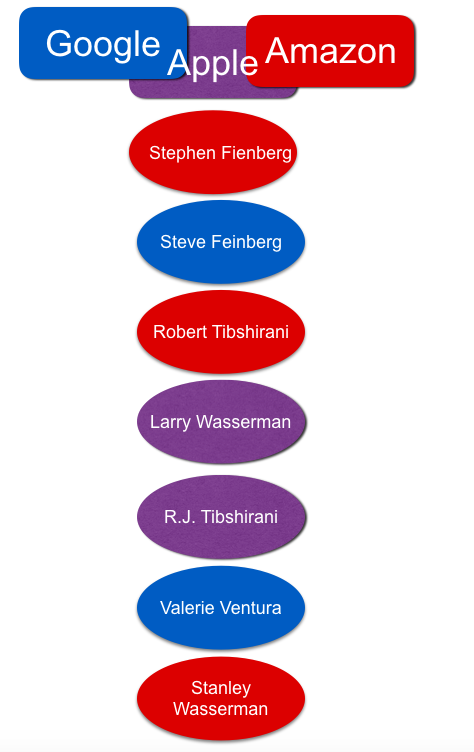
\includegraphics[scale=0.3]{figures/dedup}
%\caption{default}
%\label{default}
\end{center}
\end{figure}



}


\frame{
\frametitle{De-duplication}

Much of the literature can be grouped into the case of de-duplication. 

\vspace*{1em}

Common examples from both academia and industry are the following:

\vspace*{1em}

logistic regression, random forests, support vector machines, Bayesian adaptive regression trees,
and locality sensitive hashing. 

}

\frame{
\frametitle{The record linkage graph}
\begin{figure}[htbp]
\begin{center}
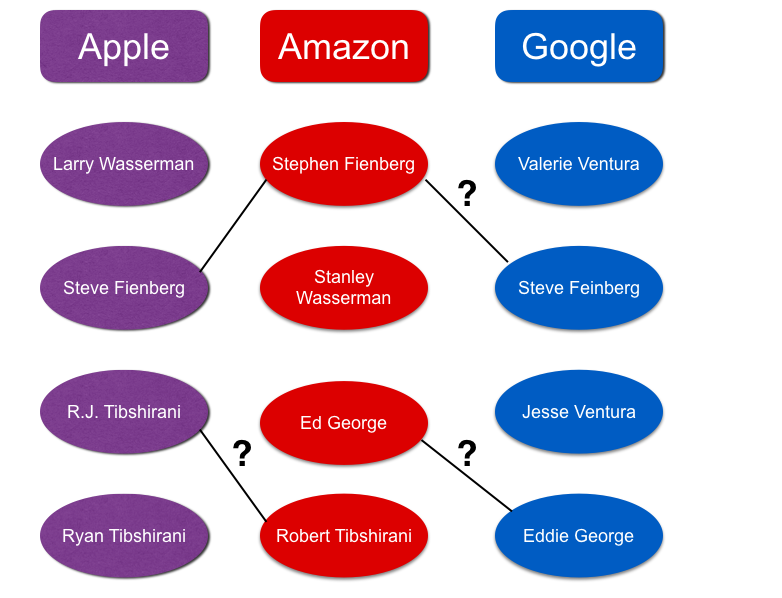
\includegraphics[scale=0.3]{figures/linkage2}
%\caption{default}
%\label{default}
\end{center}
\end{figure}

Here, we call this record linkage, since we look at the record linkage uncertainty of the entire graphical structure. 

}

%\frame{
%
%[[Walk through the code of this on my own]]
%
%How do we use logistic regression as a classification tool for record linkage? 
%\vspace*{1em}
%
%First, split the data into a training and validation set. 
%
%Then use the training data to get predictions of the following:
%%
%$$P(Y=1 \mid X) 
%= \frac{
%e^{\beta_0 + \beta^T X
%}}
%{1+e^{\beta_0 + \beta^T X
%}}$$
%
%
%
%}

\frame{
\frametitle{Blocking}
Often one performs blocking due to the fact that record linkage problems require 
a quadratic number of comparisons. 

\begin{figure}[htbp]
\begin{center}
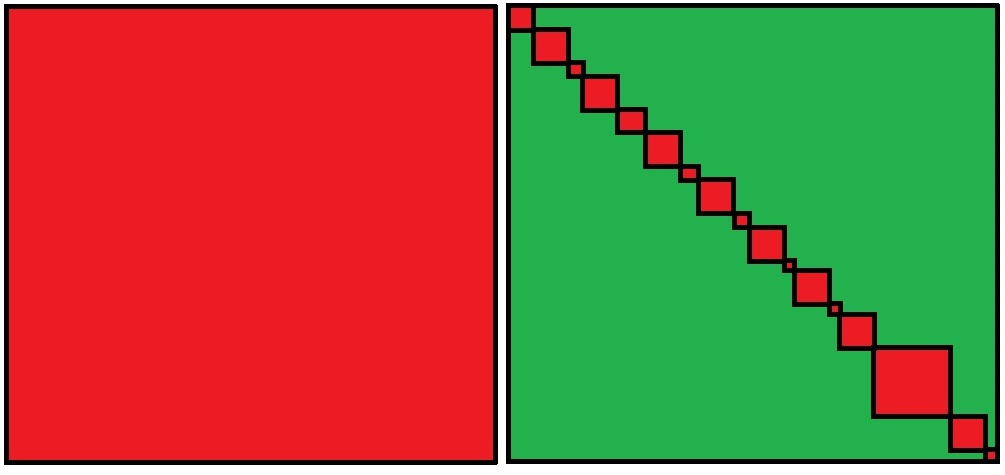
\includegraphics[width=0.5\textwidth]{figures/block}
%\caption{Not-blocking (left) versus dividing the space into partitions (left, red) and only having to run a record linkage method within each partition (right, red). }
\caption{All-to-all record comparisons (left) versus partitioning records into blocks and comparing records only within each partition (right).}
\label{block}
\end{center}
\end{figure}

We will assume some method of blocking is embedded within a record linkage procedure. 

}

\frame{
\frametitle{Blocking}

The most common method used for blocking is typically
\begin{enumerate}
\item deterministic blocking method
\item probabilistic blocking method 
\end{enumerate}

Examples include blocking on features (deterministic) or probabilistic types such as locality sensitive hashing. 

\vspace*{1em}
See Christen (2012); Steorts, Ventura, Sadinle, Fienberg (2014); Chen, Shrivastava, Steorts (2017). 
}




\frame{
\frametitle{Common Methods for Entity Resolution}


\begin{itemize}
\item Match on a unique identifier if it exists.
\item Perform exact matching.
\item Perform a likelihood ratio or hypothesis test. 
\end{itemize}

[Newcombe (1959), Fellegi and Sunter (1969)]. 

}

\frame{
\frametitle{Unique Identifier}

Suppose that each feature has a unique identifier that we are sure is accurate, like social security number. 

\vspace*{1em}

Then we can unique match records based on the unique identifier. 

\vspace*{1em}

Problems occur this unique identifier is missing or has noise in it, etc. 


}

\frame{
\frametitle{Exact Matching}

In exact matching, we compare all features. We decide if the record is a match if they agree on all features. Otherwise, we decide the record is a non-match. 

\begin{figure}[htbp]
\begin{center}
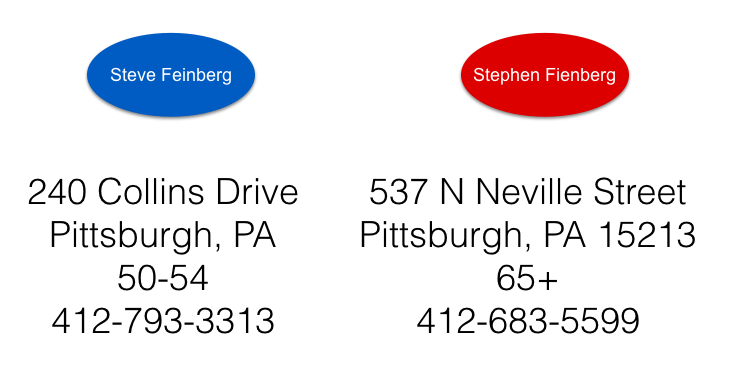
\includegraphics[width=0.8\textwidth]{figures/fienberg}
\label{block}
\end{center}
\end{figure}

Why would this method be bad for evaluation purposes?


}

\frame{
\frametitle{Fellegi and Sunter Method}
\vspace*{2em}
\begin{itemize}
\item Newcombe (1959), Fellegi and Sunter (1969): \\two databases, all-to-all comparison of records. 
\item Neyman Pearson hypothesis test with a threshold $t.$
\item If record $i$ and $j$ are above $t,$ then we have a match.
\item Otherwise, a non-match. 
\end{itemize}
}

\frame{
\frametitle{Fellegi and Sunter Method}
\begin{itemize}
\item Computationally intractable.
\item Transitivity not preserved. 
\item If 1 matches 2, and 2 matches 3, then 1 does NOT necessarily match 3. 
\end{itemize}

\textcolor{blue}{Major limitations and major flaws of this method!}




\vspace*{-4em}
\begin{figure}[htbp]
\begin{center}
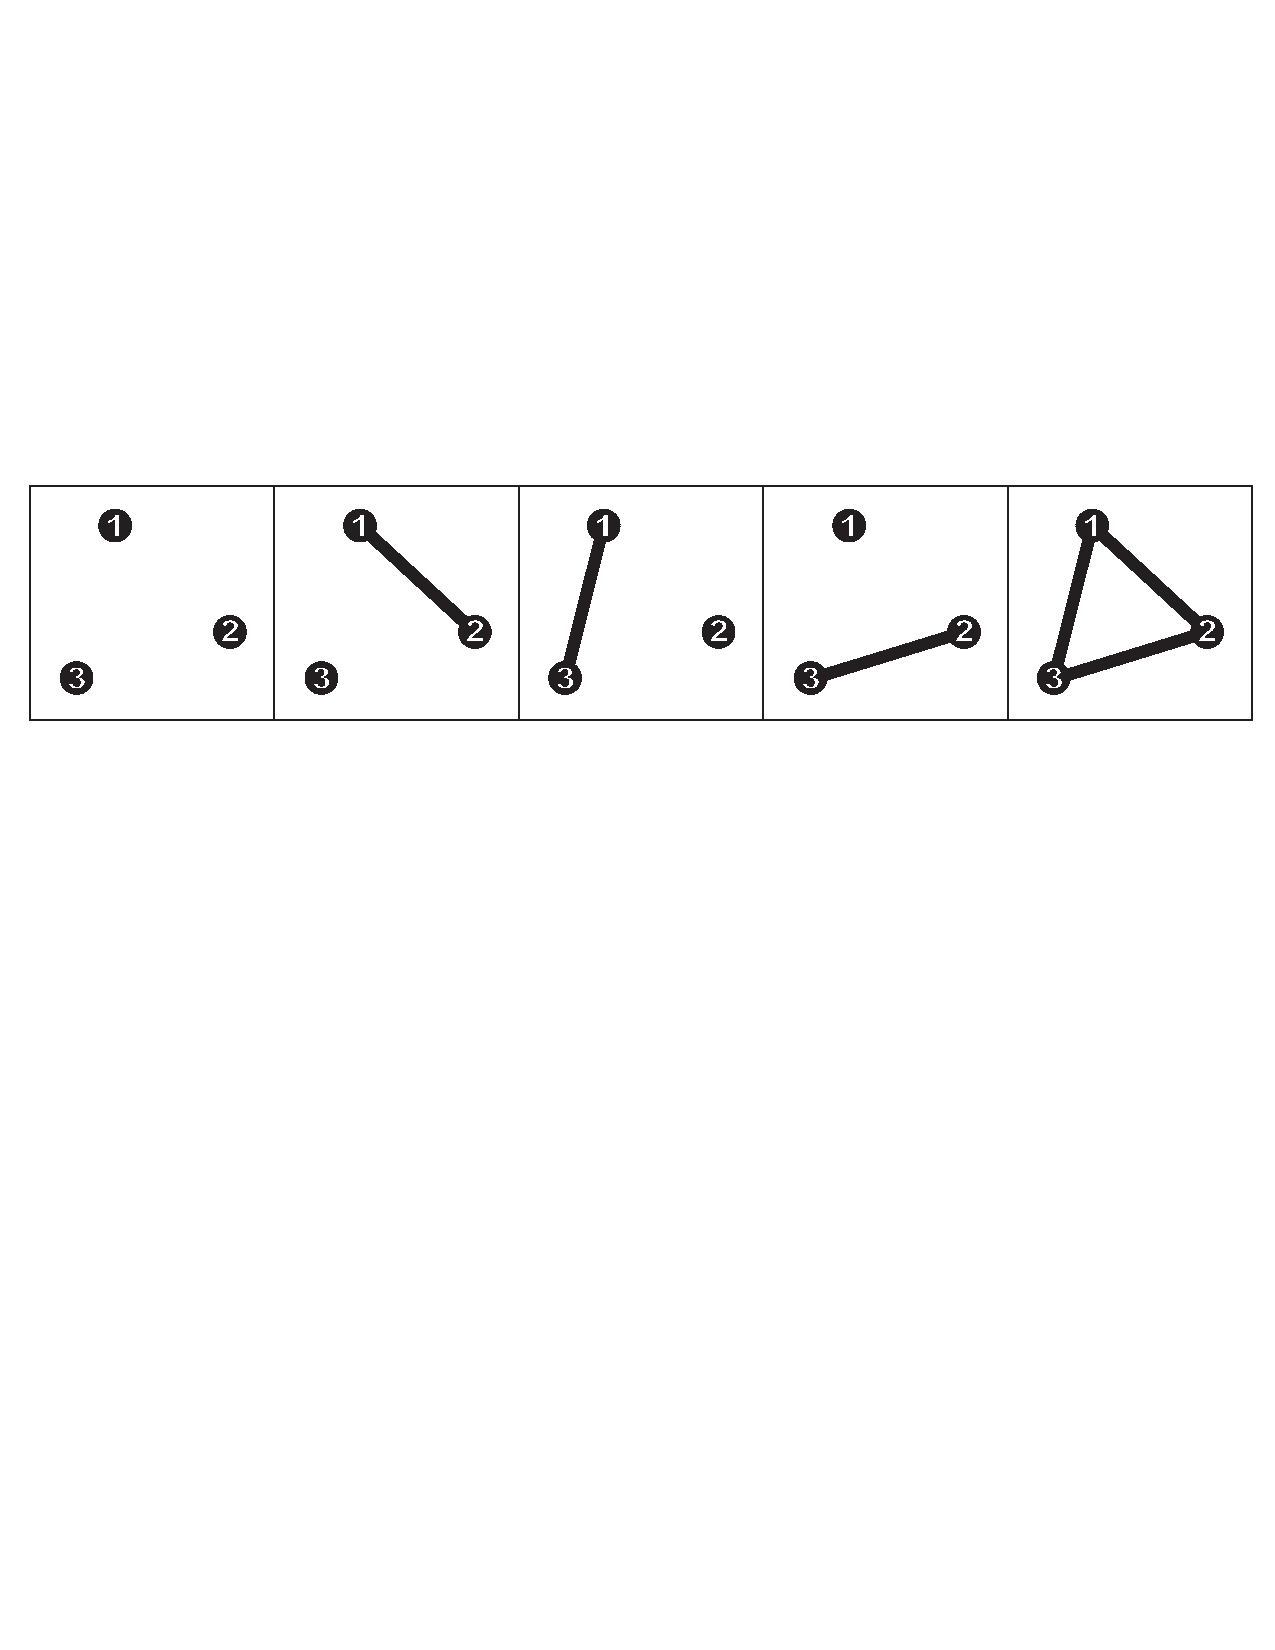
\includegraphics[width=0.8\columnwidth]{figures/transitive3.pdf}
\label{default}
\end{center}
\end{figure}


}

\frame{
\frametitle{Evaluation Metrics}

How do we evaluate performance of a particular record linkage method?

}



\frame{
\frametitle{Evaluation Metrics}

\begin{enumerate}
\item Recall
\item Precision
\item Reduction Ratio 
\item Estimated Sample Size
\item Standard Error of Estimated Sample Size
\item Run Time
\item Robustness to Tuning Parameters
\item Do Supervised Methods Overfit the Data
\end{enumerate}

}

\frame{
\frametitle{Evaluation Metrics}
\begin{enumerate}
\item  Pairs of data can be linked in both the handmatched
training data (which we refer to as ``truth") and under the estimated
linked data. We refer to this situation as true positives (TP). 
\item Pairs of data can be linked under the truth but not linked under the estimate, which
are called false negatives (FN). 
\item Pairs of data can be not linked under the truth but linked under the estimate, which are called false positives (FP). 
\item  Pairs of data can be not linked under the truth and also not linked
under the estimate, which we refer to as true negatives (TN).
\end{enumerate}


}

\frame{
\frametitle{Recall, Precision, Reduction Ratio}

$$\text{Recall} = \frac{FN}{TP + FN} = 1 - FNR.$$\\
\pause
$$\text{Precision} = \frac{FP}{TN + FP} = 1 - FPR.$$\\

\pause

\vspace{1em}

Reduction ratio (RR) measures the relative reduction of the comparison space from the de-duplication or hashing technique. 

\vspace*{1em}

See Christen (2012), Steorts, Ventura, Sadinle, Fienberg (2014) for a formal definition. 

}

\frame{
\frametitle{Other Evaluation Metrics}

\begin{enumerate}
\item Estimated Sample Size 
\item Standard Error of Estimated Sample Size
\item Run Time
\item Robustness to Tuning Parameters
\item Do Supervised Methods Overfit the Data
\end{enumerate}

\begin{enumerate}
\item The estimated sample size and standard error must be defined for each method, but this is not difficult to do in practice. 
\item Any method can be evaluated also for the run time, so one can gauge computationally costs. 
\item Robustness of tuning parameters should be explored from a Bayesian and a frequentist perspective. 
\item It's also essential to make sure that supervised methods do not overfit the data (see Steorts (2015)). 
\end{enumerate}
}

\frame{
\frametitle{RLdata500 dataset}

Let's look at an example on data that is available from the Record Linkage package in R, where we compare many different methods according to the evaluation metrics that we have laid out. 

\vspace*{1em}

We will first describe the data set and then compare the following methods in R:
\vspace*{1em}

\begin{enumerate}
\item blink
\item logistic regression 
\item random forests
\item Bayesian adaptive regression trees
%\item support vector machines
\end{enumerate}

}

\begin{frame}[fragile]
\frametitle{RLdata500 dataset}

\begin{verbatim}
  fname_c1 fname_c2 lname_c1 lname_c2   by bm bd
1  CARSTEN     <NA>    MEIER     <NA> 1949  7 22
2     GERD     <NA>    BAUER     <NA> 1968  7 27
3   ROBERT     <NA> HARTMANN     <NA> 1930  4 30
4   STEFAN     <NA>    WOLFF     <NA> 1957  9  2
5     RALF     <NA>  KRUEGER     <NA> 1966  1 13
6  JUERGEN     <NA>   FRANKE     <NA> 1929  7  4
\end{verbatim}

The \texttt{RLdata500} data set consists of 500 records with 10 percent duplication. 
\end{frame}



%\frame{
%\frametitle{RLdata500 dataset}
%
%Make comparisons regarding the recall, precision, RR, estimated K, SE. 
%Tuning parameters and sensitivity analysis is harder since we need to do this for each method. 
%Perhaps do this for just one method. 
%
%}

\frame{
\begin{figure}[ht]
\begin{minipage}[t]{0.45\linewidth}
\centering
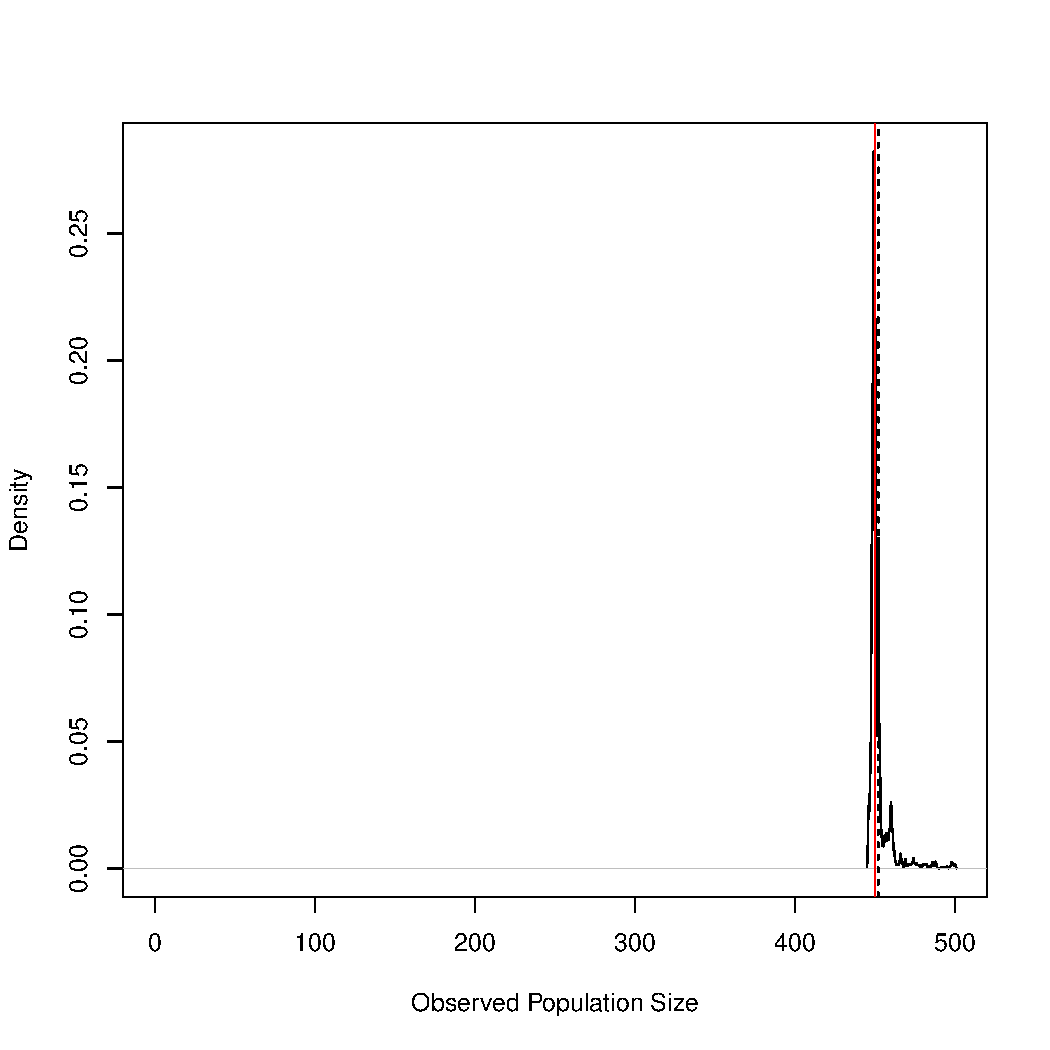
\includegraphics[scale=0.3]{figures/posterior_5000_v5_distort_1percent.pdf}
\caption{Posterior density for N in simulation study. The FNR and FPR:  0.04 and  0.02. 
%The posterior mean and standard error are 473 and 10.  
%The code used to produce this plot was $\texttt{RL\_gibbs-20140120\_v6.R}$. The total run time is 2.5 hours. 
}
\label{fig:figure1}
\end{minipage}
\hspace{0.5cm}
\begin{minipage}[t]{0.45\linewidth}
\centering
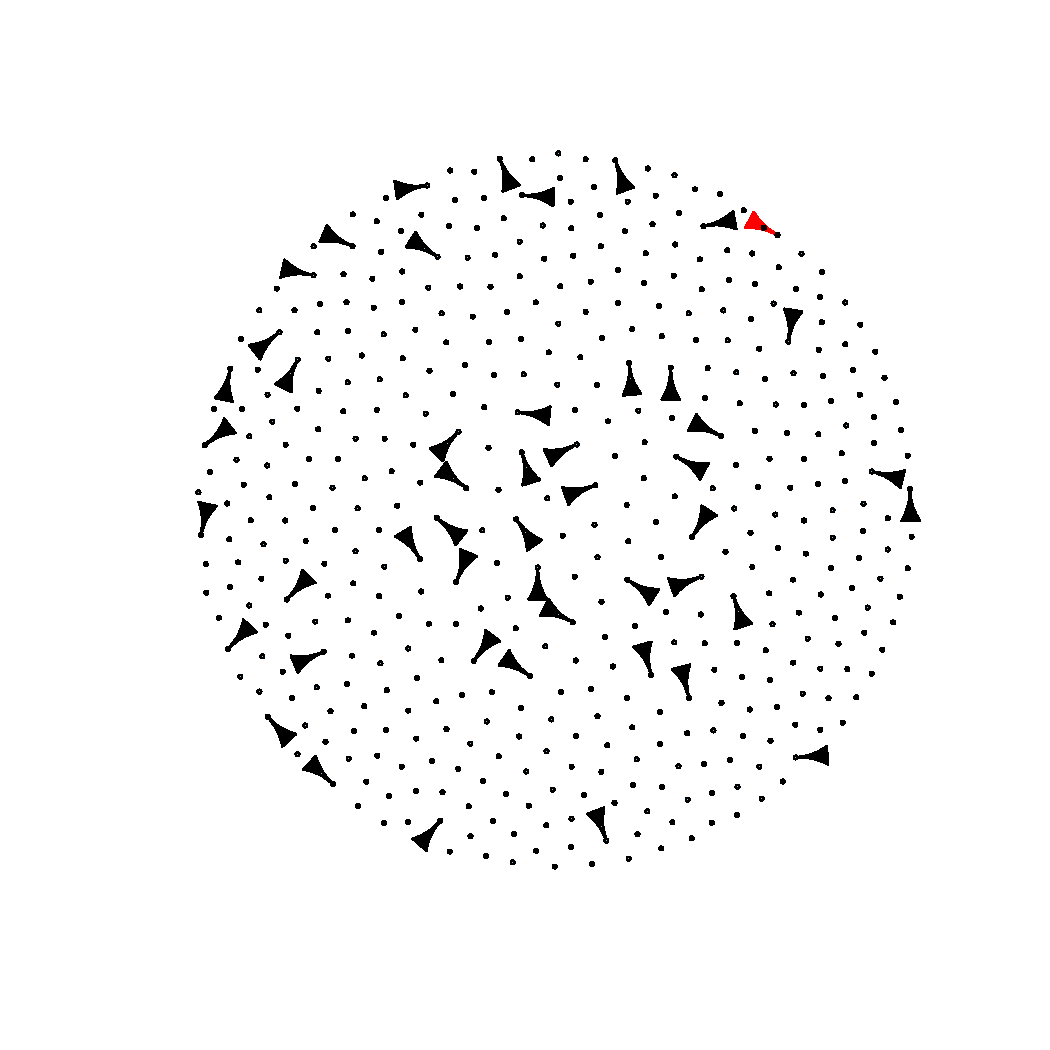
\includegraphics[scale=0.3]{figures/network_EB_5000_v5_1percent_distortion.pdf}
\caption{Shared MPMMS graphical representation of simulation study.  Only makes one false positive set.
% The algorithm only makes one false positive set consistent with the FPR being 0.02.
% The code used to produce this plot was $\texttt{RL\_gibbs-20140120\_v6.R}$.
}
\label{fig:figure2}
\end{minipage}
\end{figure}


}

\frame{
\small
\begin{table}[h]
\centering
\begin{tabular}{lcc}\toprule
Procedure&FNR&FDR\\\midrule
blink (Steorts (2015))&0.02&0.08\\
Exact Matching&1&0\\
Near-Twin&1&0\\
BART (10\% training)&0.10&0.16\\
BART (20\% training)&0.07&0.11\\
BART (50\% training)&0.03&0.04\\
BART (full data)&0.02&0\\
%Random Forests&0.04&0.08\\
Random Forests (10\% training)&0.05&0.15\\
Random Forests (20\% training)&0.04&0.09\\
Random Forests (50\% training)&0.02&0.06\\
Random Forests (full data)&0.04&0.06\\
Logistic Regression (10\% training)&0.09&0.16\\
Logistic Regression (20\% training)&0.06&0.07\\
Logistic Regression (50\% training)&0.02&0.01\\
Logistic Regression (full data)&0.02&0\\
\bottomrule
\end{tabular}
\caption{False negative rate (FNR) and false discovery rate (FDR) for the proposed EB methodology and five other record linkage methods. For the supervised methods, we
run 100 iterations of each one and average these such that overfitting is not occurring. 
}
%The \texttt{blink} method produces very low FNR and FDR compared to the supervised learning methods.
% }
%We see that each supervised method is sensitive to how much training data is used, which is not desirable and that often \emph{both} low FNR and FDR cannot be achieved for the supervised methods.}
\label{tab:fnr-fdr-rldata500}
\end{table}

}

\frame{
\frametitle{Robustness}

How do we make sure a method is robust?

\vspace*{1em}

For a semi-supervised method, we want to make sure that it's robust to different choices of the training/test data and any tuning paramater(s). 

\vspace*{1em}

For probabilistic and Bayesian methods, we want to make sure these methods are robust to choices of hyper-parameters and/or tuning parameters. 

\vspace*{1em}

Robustness, computational time complexity, and sensitivity analysis can be further explored in Steorts (2015) and Steorts, Hall, Fienberg (2016). 

}

\frame{
\frametitle{What Record Linkage Needs}

\begin{enumerate}
\item Workshops and Forums 
\item Open Source Software
\item Reproducibility and Fairness
\item Evaluation Metrics and Comparisons
\item Transparency 
\item Ethical Use of Data
\item Proper Privacy Protections of Sensitive Data
\end{enumerate}



}

%\frame{
%
%Let's turn back to our motivating application of the US Census or the Syrian conflict. How would we estimate the sample and standard error in practice?
%
%}

%\frame{
%
%Suppose that we have a total of $M$ records in $D$ data sets. 
%
%\begin{enumerate}
%\item We seek models that are much less than $O(M^2)$ (quadratic).
%\item We seek models that are reliable, accurate, fit the data well, and account for the uncertainty of the model.
%\end{enumerate}
%
%\pause
%These two goals fundamentally go against one another, making entity resolution a very challenging problem.
%\vspace*{1em}
%
%
%\pause
%In order to solve the problem at hand, we will solve a slightly easier problem, where we simply provide an estimate and standard error of the documented identifiable deaths. 
%\vspace*{1em}
%
%\pause
%
%We refer to this subtask of entity resolution as unique entity estimation. 
%
%}
%
%\frame{
%\frametitle{Our Contributions}
%
%\begin{enumerate}
%\item We formalize unique entity estimation as approximating the number of connected components in a graph with sub-quadratic  computational time. 
%\item Our proposed methodology makes no assumptions regarding the generating process of the records and gives an estimate in sample (with standard errors). 
%\item Our proposal leverages locality sensitive hashing (LSH) in a novel way for the estimation process, where our estimator is unbiased and has provably low variance compared to random sampling based approaches. 
%\item We apply our method to official statistics data, music data, food data, and a subset of the ongoing conflict in Syria. 
%\end{enumerate}
%
%Chen, Shrivastava, \textbf{RCS} (2018), AoAS (Minor Revision), \url{https://arxiv.org/abs/1710.02690},\\
% \href{https://github.com/keroro824/RL_data/blob/master/README}{Code Link}
%
%}
%
%\frame{
%\frametitle{Fast Unique Entity Estimation}
%
%\begin{figure}[htbp]
%\begin{center}
%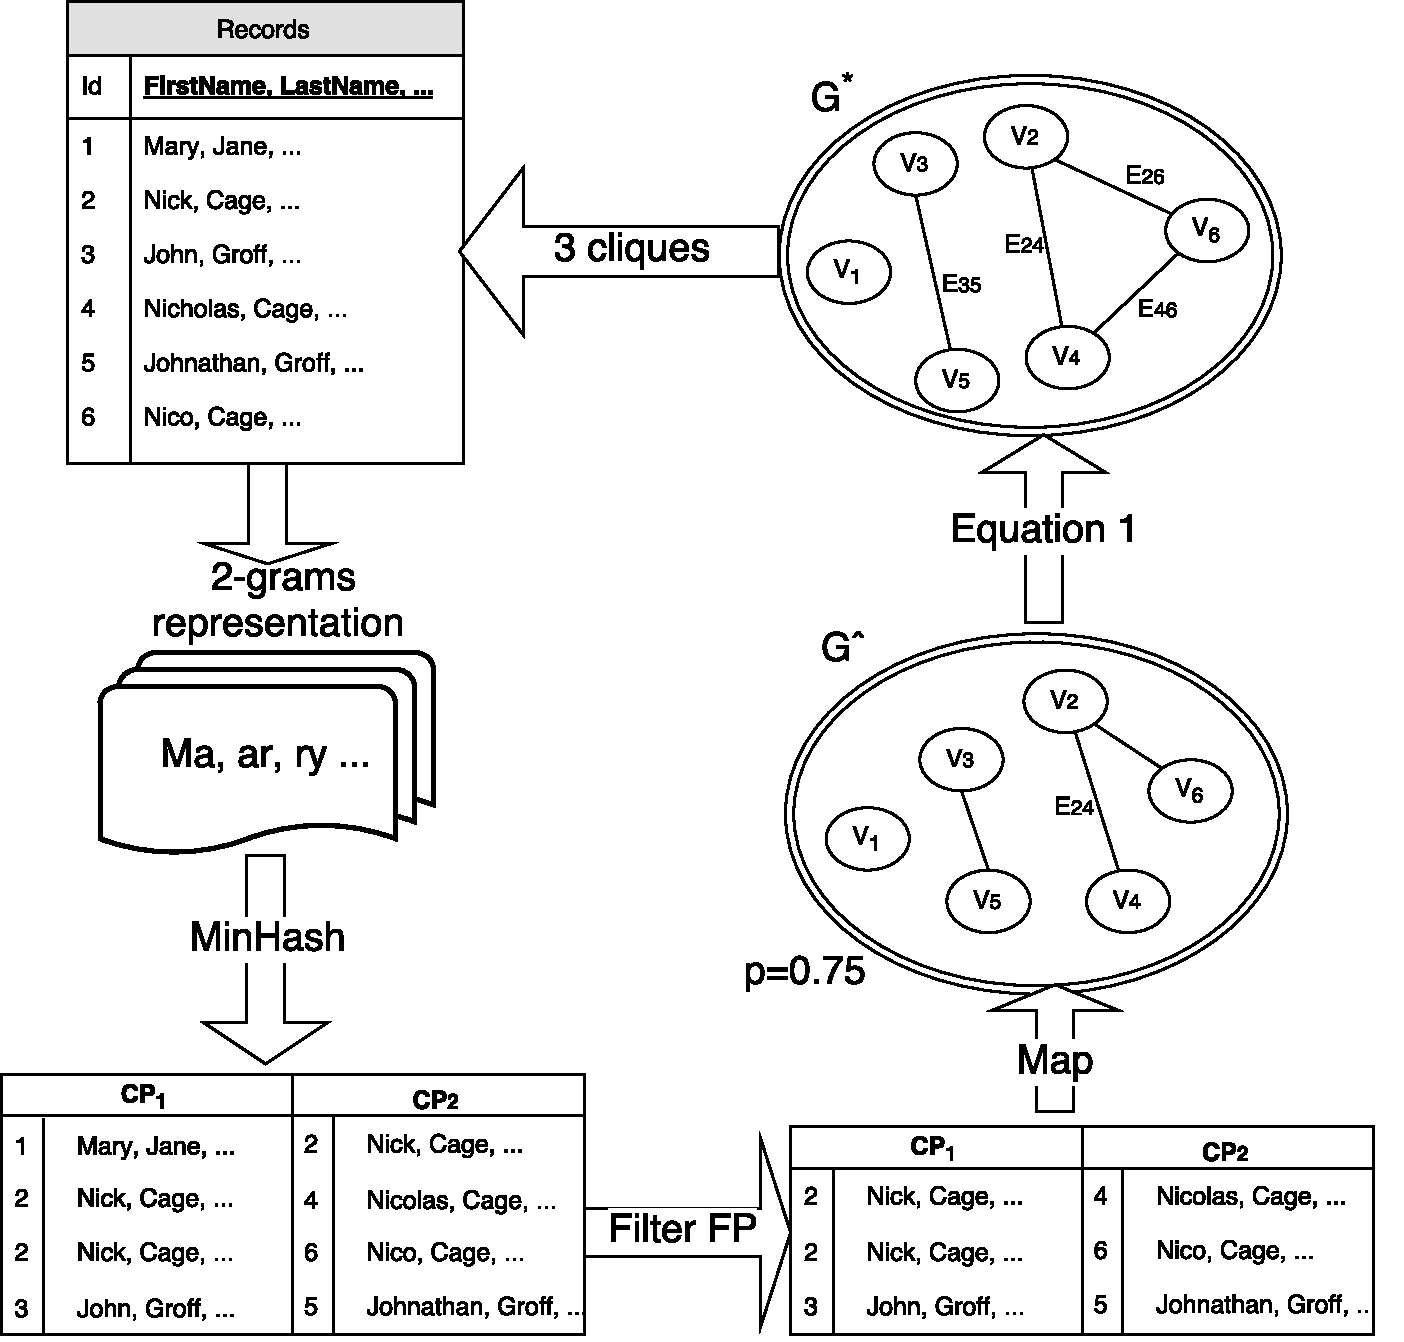
\includegraphics[width=0.7\textwidth]{figures/flow}
%%\caption{default}
%\label{default}
%\end{center}
%\end{figure}
%
%
%}
%
%\frame{
%\frametitle{Applications}
%
%The proposed method is applied to three real applications, with comparisons to standards in the literature. 
%
%\begin{table}[t]
%	\caption{ presents five important features of the four data sets.
%%	(three well-labeled real data set and Syrian data set).
%	\textbf{Domain} reflects the variety of the data type we used in the experiments. \textbf{Size} is the number of total records respectively. \textbf{\# Matching Pairs} shows how many pair of records point to the same entity in each data set. \textbf{\# Attributes} represents the dimensionality of individual record. \textbf{\# Entities} is the number of unique records.}
%	\label{table1}
%	\centering
%	\tiny
%				
%	\begin{tabular}{lccccc}
%		\toprule
%		\textbf{DBname} & \textbf{Domain}& \textbf{Size} & \textbf{\# Matching Pairs} & \textbf{\# Attributes}& \textbf{\# Entities} \\
%		\midrule
%		Restaurants & Restaurant Guide&864  &112 & 4&752 \\
%	
%		CD & Music CDs&9,763  &299 & 106 & 9,508\\
%	
%		Voter & Registration Info&324,074  & 70,359 & 6 & 255,447\\
%	
%		Syria & Death Records&296,245  & N/A & 7 & N/A\\
%		\bottomrule
%	\end{tabular}	
%\end{table}
%
%
%}
%
%
%\frame{
%\frametitle{Results}
%
%\begin{figure}[htbp]
%\begin{center}
%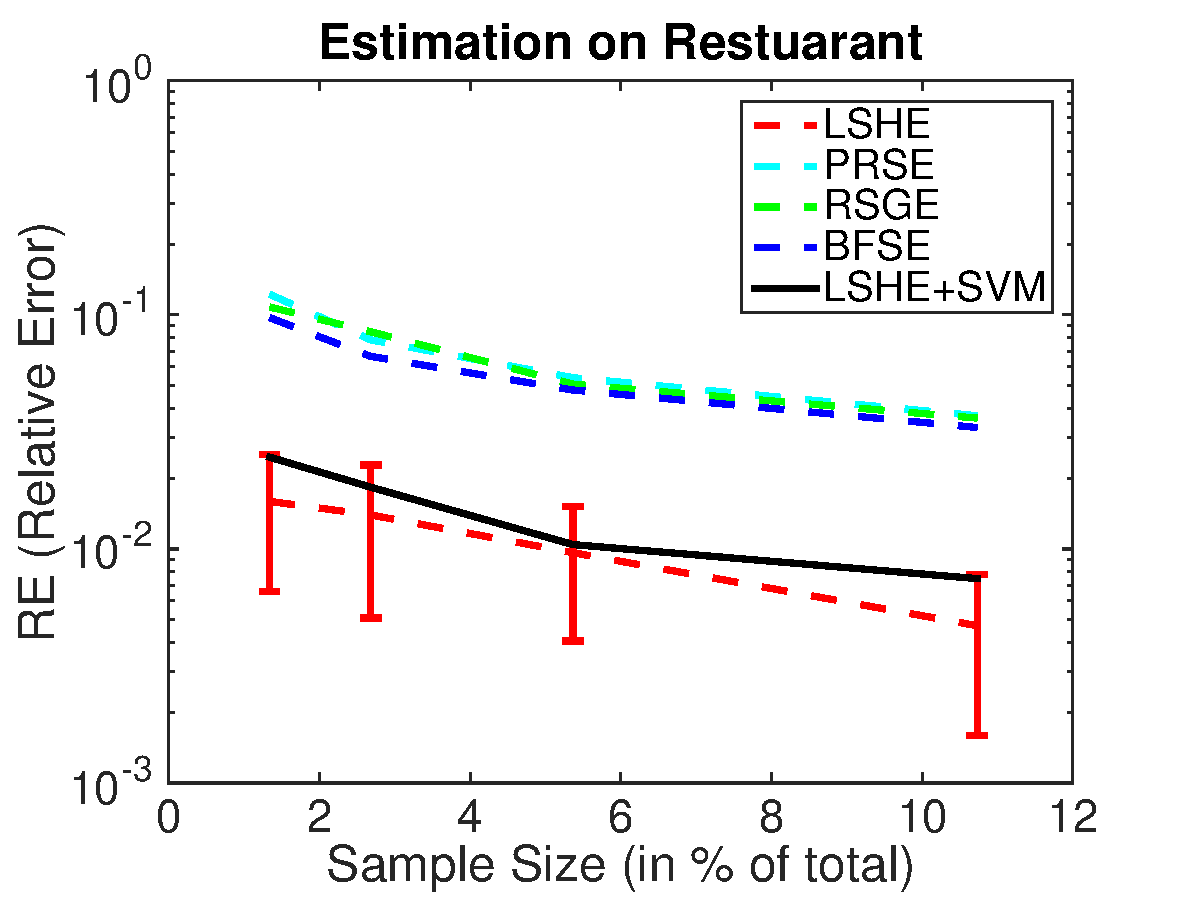
\includegraphics[width=0.7\textwidth]{figures/restaurant}
%%\caption{In its third report on Syria commissioned by the United Nations, the Human Rights Data Analysis Group identified 191,369 deaths from the start of the conflict in March 2011 to April 2014, more than double the 92,901 deaths cited in the group?s last report, which covered the first two years of the conflict.}
%\label{default}
%\end{center}
%\end{figure}
%
%\begin{itemize}
%\item Our methods: Red (LSHE) and black (LSHE + SVM) 
%\item Comparisons: blue and green (random sampling)
%\end{itemize}
%
%
%}
%
%\frame{
%\frametitle{Results}
%
%\begin{figure}[htbp]
%\begin{center}
%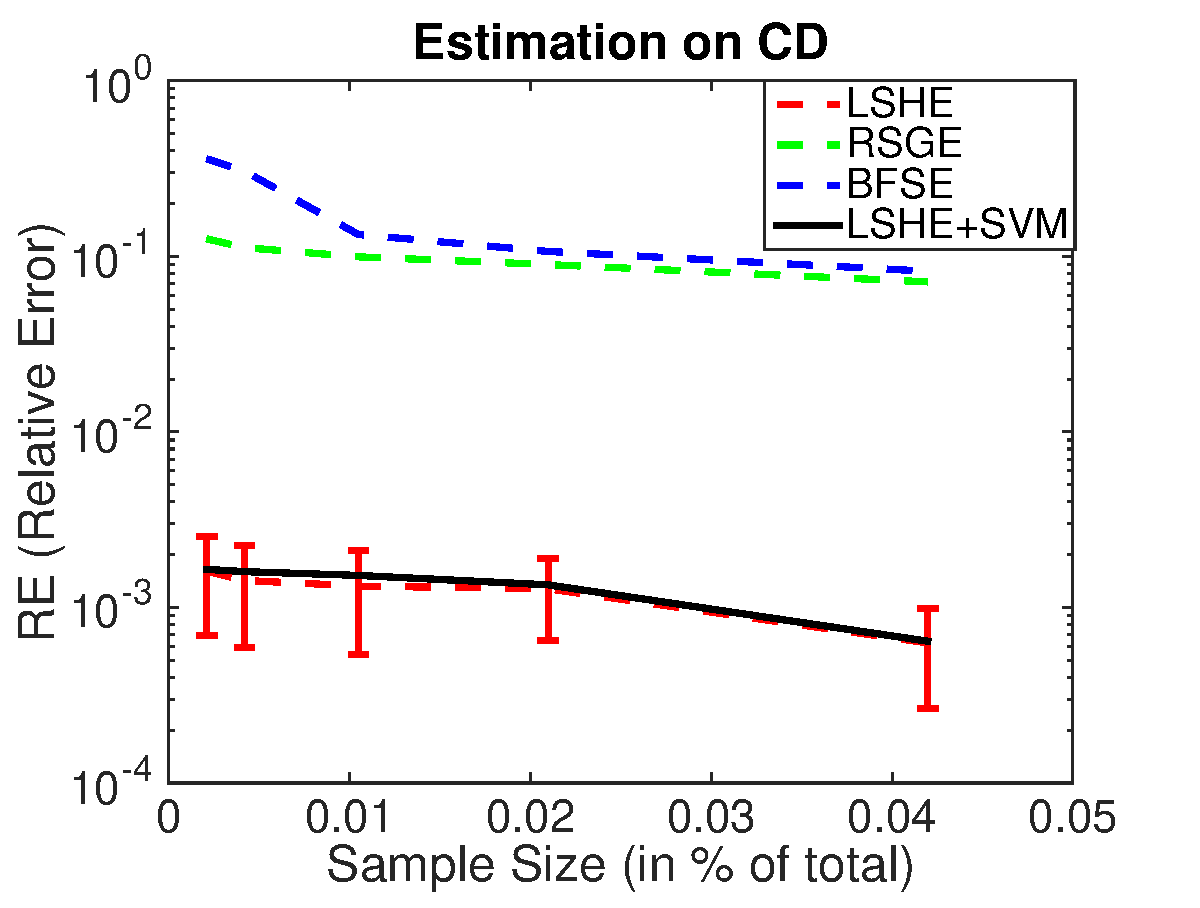
\includegraphics[width=0.7\textwidth]{figures/cd}
%%\caption{In its third report on Syria commissioned by the United Nations, the Human Rights Data Analysis Group identified 191,369 deaths from the start of the conflict in March 2011 to April 2014, more than double the 92,901 deaths cited in the group?s last report, which covered the first two years of the conflict.}
%\label{default}
%\end{center}
%\end{figure}
%
%\begin{itemize}
%\item Our methods: Red (LSHE) and black (LSHE + SVM) 
%\item Comparisons: blue and green (random sampling)
%\end{itemize}
%
%
%}
%
%\frame{
%\frametitle{Results}
%
%\begin{figure}[htbp]
%\begin{center}
%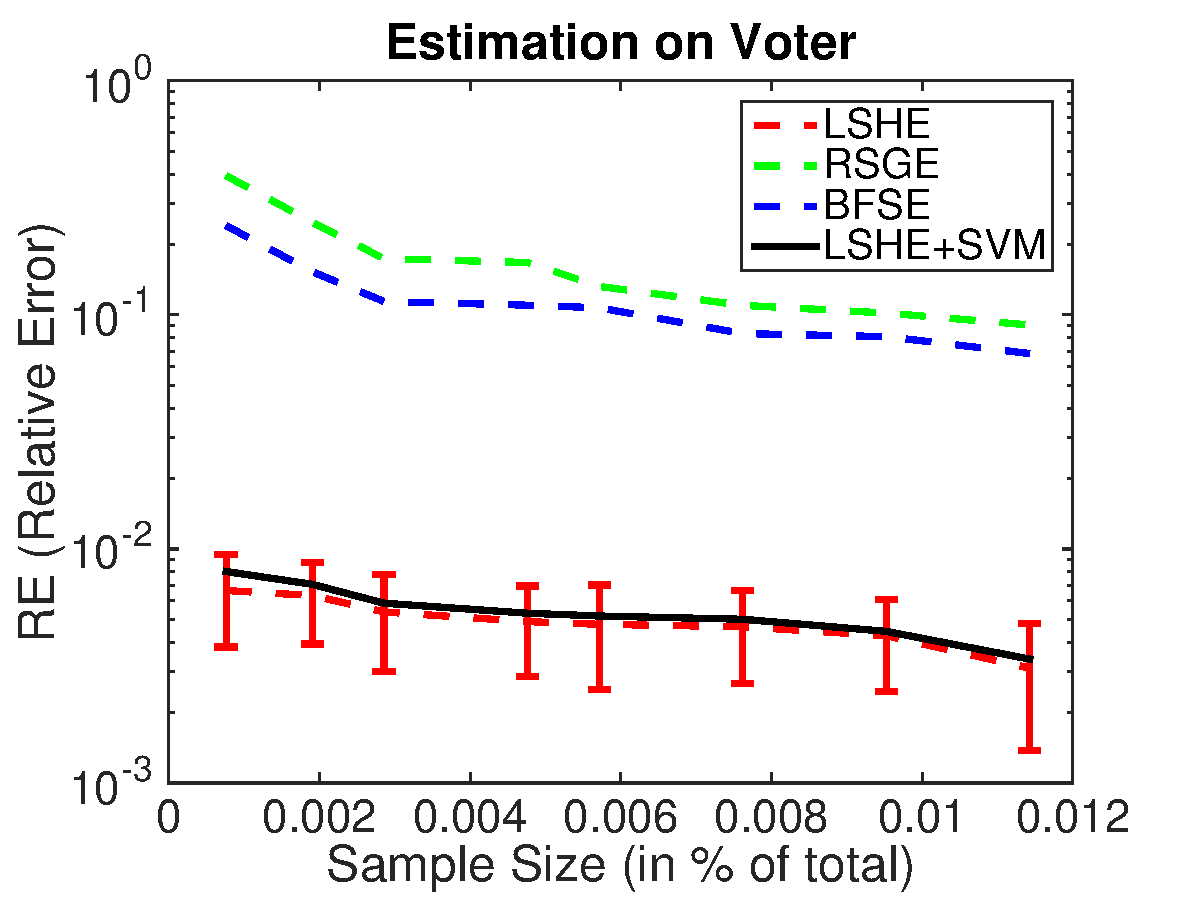
\includegraphics[width=0.7\textwidth]{figures/voter}
%%\caption{In its third report on Syria commissioned by the United Nations, the Human Rights Data Analysis Group identified 191,369 deaths from the start of the conflict in March 2011 to April 2014, more than double the 92,901 deaths cited in the group?s last report, which covered the first two years of the conflict.}
%\label{default}
%\end{center}
%\end{figure}
%
%\begin{itemize}
%\item Our methods: Red (LSHE) and black (LSHE + SVM) 
%\item Comparisons: blue and green (random sampling)
%\end{itemize}
%
%
%}
%
%\frame{
%\frametitle{Syrian data set}
%
%\begin{itemize}
%\item Using our proposed methodology, used 917,577 sampled pairs and then used an SVM for classification of matches and non-matches. 
%\item After looking at a sensitivity analysis of the tuning parameters for our proposed method, we report that there are 191,874 documented identifiable deaths, with standard deviation of 1,772, which is very close to HRDAG's estimate of 191,369 in Price et al. (2014).
%\item Furthermore, we also report the recall (false positives) = 0.83 and the precision (false negatives) = 0.99. 
%\item Finally, one iteration of the method takes only 127 seconds!  
%\end{itemize}
%
%
%}




%\frame{
%\frametitle{Summary}
%
%
%\begin{enumerate}
%
%
%
%\end{enumerate}



%}

\frame{
\center
Thank you!  Questions?\\

\vspace*{1em}

Thank you to the National Science Foundation for NSF CAREER Microclustering and NSF Big Data Privacy. The views in this talk are of the authors alone and not of the funding organization. \\

\vspace*{1em}



Contact: beka@stat.duke.edu\\
Webpage: resteorts.github.io\\
(All papers and software can be found above).

}



\end{document}